%%notwendige packages

%----------------------------

\documentclass[12pt]{article}
%benötigt man immer
\usepackage{amsmath}
%is used for numbering of equations
\usepackage[english]{babel}
\usepackage[utf8x]{inputenc}
\usepackage{varwidth}
\usepackage{float}
% Table caption on top of tables
\floatstyle{plaintop}
\restylefloat{table}
%----
\usepackage{makecell}
\usepackage{enumitem}

% allows index generation
\usepackage{makeidx}
\makeindex

% equation, table and figure numbering should start with section number e.g. (3.1)
\numberwithin{equation}{section}
\numberwithin{table}{section}
\numberwithin{figure}{section}

%fonts
\usepackage[T1]{fontenc}
\usepackage{textcomp}
\usepackage{mathptmx}
\usepackage{tabularx}
\usepackage{multirow}
\usepackage{enumitem}
%small fonts for captions of figures and tables
\usepackage{caption}
\captionsetup[figure]{font = footnotesize}
\captionsetup[table]{font = footnotesize}


%format
% Witwen und Waisenkinder vermeiden
\clubpenalty=4500	% Waisen vermeiden (erste Zeile eines neuen Absatzes als letzte Zeile einer Seite)
\widowpenalty=10000	% keine Witwen zulassen (letzte Zeile eines Absatzes am Beginn einer neuen Seite)

% Seitenraender einstellen
\usepackage{geometry}
\geometry{a4paper,left=30mm,right=20mm, top=20mm, bottom=20mm}

% Zeilenabstand
\linespread{1.5} 

%Graphics
\usepackage[final]{graphicx} 	
\usepackage[twoside,figuresright]{rotating}
\usepackage{subcaption} 
%\usepackage{subfigure} 

% Adjust tables (and figures) to textwidth...
\usepackage{adjustbox}

%For tables, to color whole row without missing pieces...
\usepackage{tabularx}
%\usepackage[table]{xcolor}  % option loads »colortbl«

% Initialize Makro for table heads
\renewcommand\theadfont{\bfseries\sffamily}

% Highlighting rows, columns and headers of tables
\usepackage{color, colortbl}
\definecolor{Gray}{gray}{0.9}
\definecolor{LightCyan}{rgb}{0.88,1,1}
\definecolor{SeaBlue}{rgb}{0.3, 0.58, 1}

%acronym package for Abbreviations
\usepackage{acronym}

%Create Statutory Declaration page for signatures
\newcommand{\namesigdate}[2][3cm]{%
  \begin{tabular}{@{}p{#1}@{}}
    #2 \\[2\normalbaselineskip] \hrule \\[0pt]
    {\small \textit{Signature}}
  \end{tabular}
}

%----------------------------

\begin{document}

\thispagestyle{empty}	
% !TEX root = Master.tex

%titlepage
\thispagestyle{empty}
\begin{center}


\begin{minipage}{0.75\linewidth}
    \centering
%University logo
    
\includegraphics[scale = 0.7]{figures/uni_goettingen_logo.pdf}\\
    
    %\rule{0.4\linewidth}{0.15\linewidth}\par
    \vspace{1cm}
    
% Master Thesis
{{\Huge \textbf{Master Thesis} \par}}
    
\vspace{0.5cm}
    
%Thesis title
    {{\LARGE Multivariate modelling of the dependency structure between article sales of a sportswear manufacturer\par}}
    \vspace{1cm}
    
    
%Author's name
\begin{center}
Author\\
{\LARGE \textbf{Petros Christanas}} \\


\vspace{0.5cm}

Matriculation Number \\
{\large 11604278}

\vspace{1cm}

{\Large Student of Applied Statistics M.Sc.}\\
{\large Chair of Statistics and Econometrics}

\end{center}
    
    \end{minipage}
\end{center}


\vspace{2cm}

\noindent Supervisors\\
\noindent {\Large \textbf{Prof. Dr. Thomas Kneib}} \\
\noindent {\Large \textbf{Der andere}} \\

\vspace{1cm}
    
%Date
\begin{flushleft}
\noindent {\Large \today}
\end{flushleft}

    
    

\clearpage
%\clearpage
\newpage
\null\thispagestyle{empty}
\newpage
\thispagestyle{empty}
\section*{Statutory Declaration}
% !TEX root = Master.tex

\vspace{2cm}

I hereby declare that I wrote this thesis paper
independently, without assistance from external parties, and without use of other resources than
those indicated. All information taken from other publications or sources in text or in meaning
are duly acknowledged in the text. The written and electronic forms of the thesis paper are the
same. I give my consent to have this thesis checked by plagiarism software.

\vspace{5cm}

Nuremberg, \today


\vspace{2cm}


\noindent\begin{tabular}{ll}
\makebox[2.5in]{\hrulefill} \\
Petros Christanas \\
\end{tabular}

\newpage
\null\thispagestyle{empty}
\newpage
\thispagestyle{empty}
\section*{Acknowledgments}
% !TEX root = Master.tex

\vspace{3cm}



I would like express my deepest gratitude towards Dr. Alexander März, who guided me throughout this thesis with his expertise and is always finding the time to help during this special times. I would also like to thank the entire adidas Data Science \& AI team for contributing a great deal to my learning journey and giving me the opportunity to conduct this thesis.\\
I am also sincerely grateful towards Prof. Dr. Thomas Kneib for supervising my Master thesis and moreover for leading the study program of Applied Statistics and passing on his knowledge to his students in the best way possible.\\
Last but not least, I would like to thank my fellow students Patrick Neff and Malte Lehna who were playing a key role in my personal growth and with whom I had an unforgettable time in Göttingen. 

\vspace{1.5cm}


\textbf{\textgreekfont{Ευχαριστώ θερμά τους γονείς μου για την άνευ όρων υποστήριξη. Σας αγαπώ!}}



\newpage
\null\thispagestyle{empty}
\newpage


	
%\pagenumbering{Roman} 	
\thispagestyle{empty}
\tableofcontents
\newpage




\newpage

\pagenumbering{arabic} 
\setcounter{page}{1} 

\section{Introduction}
% !TEX root = Master.tex


Write in general something like an "abstract", what is the pipeline of the thesis as a whole..

Quick test for user specified compiling and citing:\\
\cite{lutkepohl1996specification}\\
\citep{Rcoreteam}\\
\cite{Rcoreteam}\\




\clearpage
\section{Study Area \& Data Sources}
\subsection{Forest Classification}
% !TEX root = Master.tex

The study area is a private forest enterprise in Gartow (Niedersachsen) Germany. It measures around 5674.2 ha in total (see Table \ref{tab:sizes}) and is a relatively homogenous forest consisting mostly of pine trees.

\begin{table}[H]
\setlength\arrayrulewidth{1pt}  
\centering
\begin{tabular}{|c |c |c |c|}
\hline 
\rowcolor{Gray}
\textbf{Stratum} & \textbf{Location Class} & \textbf{Area [ha]} & \textbf{Relative Area} \\ 
\hline 
1 & 1 & 338.6 & 0.06 \\ 
\hline 
2 & 2 & 1546.9 & 0.27 \\ 
\hline 
3 & 3 & 2129.3 & 0.38 \\ 
\hline 
4 & 4 & 1550.5 & 0.27 \\ 
\hline 
G & 2 & 108.9 & 0.02 \\ 
\hline 
\rowcolor{SeaBlue}
Total & - & 5674.2 & 1 \\ 
\hline 
\end{tabular} 
\caption{Size of the different stratum and associated sampling grids. Stratum 2 and G have been merged to Location Class 2 which results in an identical sampling grid.}
\label{tab:sizes}
\end{table}

The forest itself is split into stratum to take site conditions, forest structure and thus natural variation of the areas into account (see Figure \ref{fig:Gartow Map}). The assessment of variation was based on a forest inventory conducted 2008
(see Table \ref{tab:Sample_Variation}).

\begin{table}[H]
\setlength\arrayrulewidth{1pt}  
\centering
\begin{adjustbox}{max width=\textwidth}
\begin{tabular}{|c |c |c |c |c |c |c |c|}
\hline 
\rowcolor{Gray}
\textbf{Stratum} & \textbf{Location Class} & \textbf{Area [ha]} & \textbf{Relative Area} & \textbf{Sample Size} & \textbf{Mean Volume / ha} & \textbf{Sample Variance} & \textbf{SE\%} \\ 
\hline 
1 & 1 & 338.6 & 0.06 & 159 & 180.19 & 104.24 & 5.67 \\ 
\hline 
2 & 2 & 1546.9 & 0.27 & 805 & 246.75 & 22.75 & 1.93 \\ 
\hline 
3 & 3 & 2129.3 & 0.38 & 542 & 195.41 & 13.15 & 1.86 \\ 
\hline 
4 & 4 & 1550.5 & 0.27 & 134 & 131.90 & 30.45 & 4.18 \\ 
\hline 
G & 2 & 108.9 & 0.02 & 55 & 271.26 & 734.08 & 9.99 \\ 
\hline 
\rowcolor{SeaBlue}
Total & - & 5674.2 & 1 & 1659 & 196.37 & 6.46 & 1.29 \\ 
\hline 
\end{tabular} 
\end{adjustbox}
\caption{Mean volume and sample variation estimates of the forest inventory 2008. Stratum 2 and 3 show little relative standard
error (SE\%), while stratum 1 inhibits more variation. Stratum G, which covers only 2\% of the total area has a typical high variation}
\label{tab:Sample_Variation}
\end{table}

Main sources of the variation in the growing stock can be assigned by the varieties in the tree species and the age distribution of the trees. Young and therefore small trees have a smaller diameter. If an area has been cultivated around the same timespan with identical species, the trees are expected to be centred on a certain diameter. On the other hand, a very diverse area in species and time will have naturally more variation (see Figure \ref{fig:barplots_Gartow})

\begin{figure}[H]
  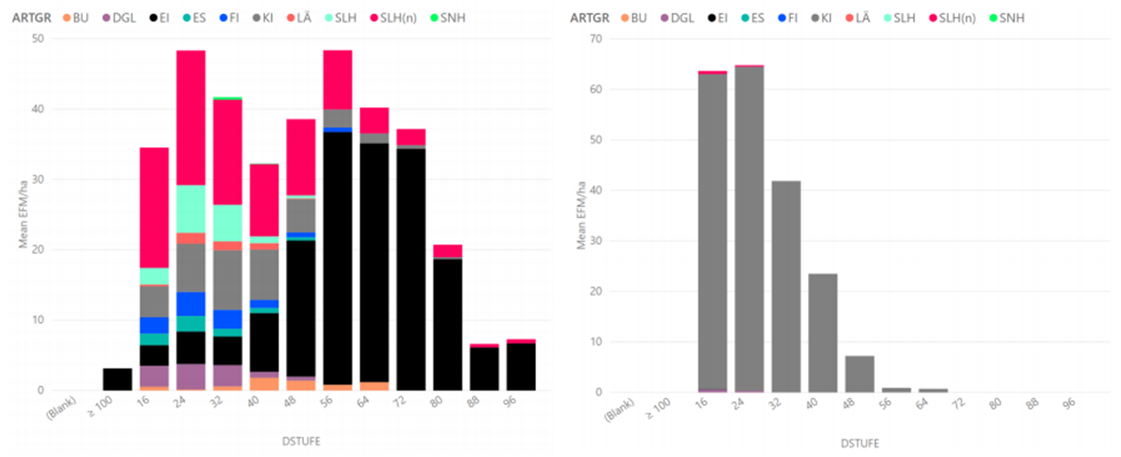
\includegraphics[width=\textwidth]{barplots_Gartow.png}
  \caption{The bar plots (left to right: stratum 1, stratum 4). The bars indicate the mean volume per ha for different diameter classes [1].}
  \label{fig:barplots_Gartow}
\end{figure}

Sampling activities are adjusting according to the inhibited variation of the stratum type (see Section \ref{Inventory Data}).

\begin{figure}[H]
  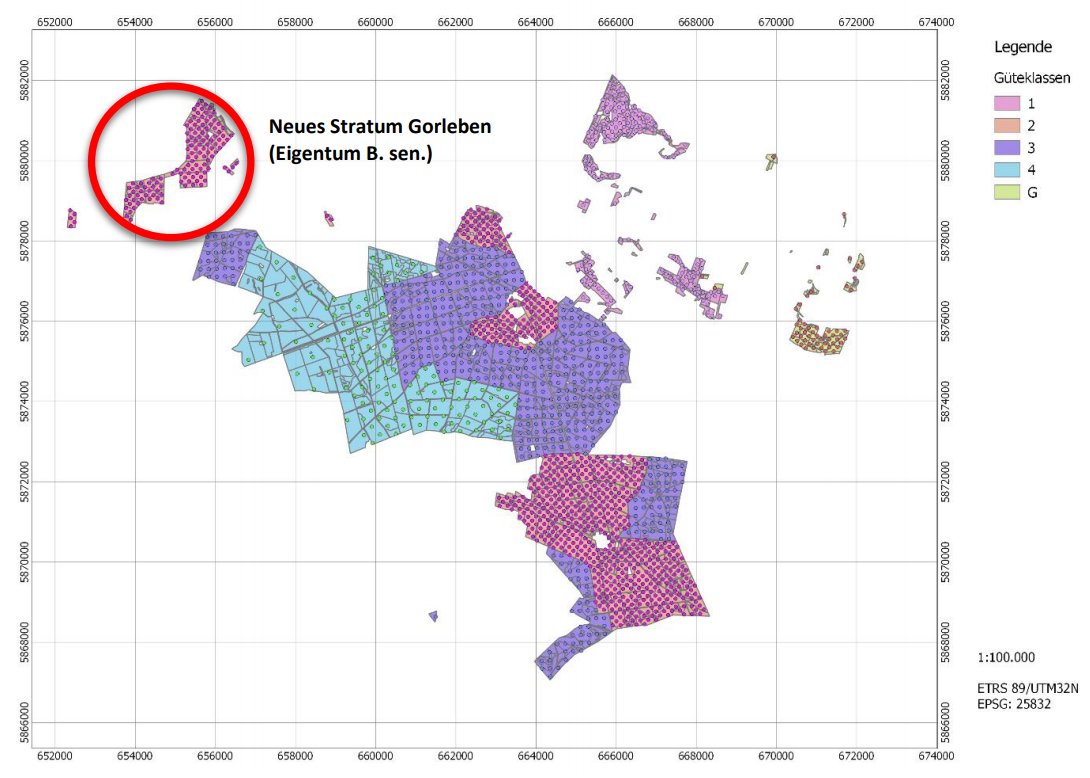
\includegraphics[width=\textwidth]{Gartow_map.png}
  \caption{The forest of Gartow is divided into stratums based on past observed variation and ownership and subdivided into compartments indicated by grey lines. Each point within a section indicate a sampling point [1].}
  \label{fig:Gartow Map}
\end{figure}

The stratum themselves are subdivided into compartments with the intention to create homogeneous sub regions (see Figure \ref{fig:Gartow Map}). The diameter distribution must be found for each of those compartments.

\subsection{Inventory Data} \label{Inventory Data}
% !TEX root = Master.tex

In spring 2018, a sample-based forest inventory was carried out in Gartow. 942 sampling locations are defined which are spread over the forest based on a stratified sampling approach. This accounts for the past observed variation within the regions. Compartments of stratum 1 and 2 are sampled with a dense sampling grid, while 3 and 4 have a wider sampling grid (see Table \ref{tab:Sample_Variation} \& Figure \ref{fig:Gartow Map}).\\

At each sampling location (so called plots) several attributes of the trees within a certain circular area are measured. The parameters of primary interest in this study are the diameter, species and height. The diameter is measured at breast height (around 1.3 meters) with a measuring tape. Subsequently, the height is measured with varying, but established methodologies. Unlike the diameter, not every tree height is collected. In each plot, three main species trees (less if there are fewer trees) are measured. To cover the total range of values, a small, a medium sized and a large one is gauged. Additionally, one tree of every other species is measured to cover the variety of species. Table \ref{tab:Measured Trees} provides an overview of total measured trees.

\begin{table}[H]
\setlength\arrayrulewidth{1pt}  
\centering
\begin{tabular}{|c| c|}
\hline 
\rowcolor{Gray}
\textbf{Stratum} & \textbf{\# Measured Trees} \\ 
\hline 
1 & 1287 \\ 
\hline 
2 & 3434 \\ 
\hline 
3 & 2734 \\ 
\hline 
4.1 & 616 \\ 
\hline 
4.2 & 792 \\ 	
\hline 
G & 523 \\ 
\hline 
GL & 619 \\ 
\hline 
\rowcolor{SeaBlue}
Total & 10005 \\ 
\hline 
\end{tabular} 
\caption{Overview of number of measured trees for height and diameter per Stratum}
\label{tab:Measured Trees}
\end{table}


\subsection{LiDAR} \label{LiDAR}
% !TEX root = Master.tex

While the previously described data will be used for modelling, data captured by the airborne LiDAR is of main interested in this report, since the ability of innovating forest inventory is discussed.\\

LiDAR uses a laser scanning system to capture distances. In context, laser scanning is referred to the active emitting and sensing of light. Thus, Light Detection and Ranging is a suitable description of the mechanics, also known as LADAR (Laser Detection and Ranging). LiDAR is a more generalized definition, as instead of laser- light also xenon or flash lamps can be used [2]. A high-level definition of the functionality of LiDAR is as follows. Laser beams are continuously emitted of the LiDAR system, mounted on an airborne vehicle. The coordinates are throughout captured by a GPS (Global Positioning System) and IMU (Inertial Measurement Unit – used to capture adjust for e.g. inclined positioning, acceleration of the vehicle). Laser or xeon/flash light is emitted of an active sensor and the distance captured once it is traveled back to the scanner. As forests have a relatively turbulent surface and only little light can reach the surface of the forest, many systems only capture the first and last impulse [3]. The cloud of captured points can then be used to create a 3-D image of the forest (see Figure \ref{fig:LiDAR}).

\begin{figure}[H]
  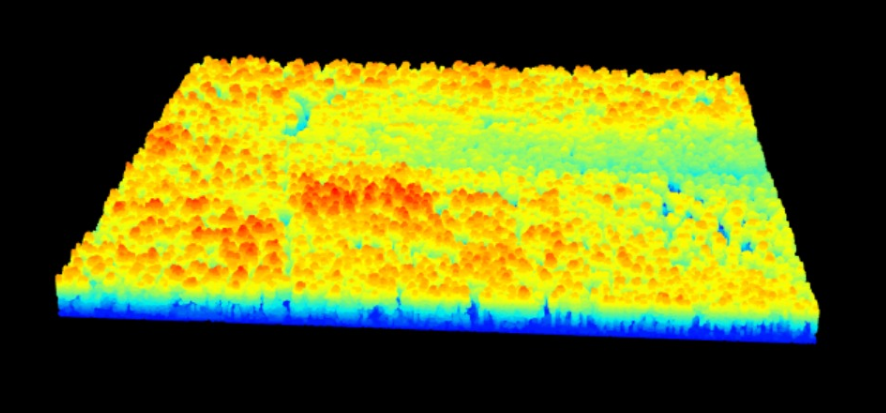
\includegraphics[width=\textwidth]{lidar.png}
  \caption{3-D Image of a small area of the forest of Gartow made by the airborne LiDAR. The determined height is colorized. A
dense group of height trees is found almost in the middle and directly behind an aisle of small trees.}
  \label{fig:LiDAR}
\end{figure}

Main benefits of LiDAR compared to other systems is the ability to capture data regardless of sun positioning, day or night and the ability to map through the highly dense areas (the canopies of the trees). The main benefit compared to the traditional way of forest inventory is relative intuitive. A plane is capable of objectively measuring the forest subject to this report in under a week; while a forester must inspect every single hectare, providing a more subjective intuition of the forest inventory.

\begin{table}[H]
\setlength\arrayrulewidth{1pt}  
\centering
\begin{adjustbox}{max width=\textwidth}
\begin{tabular}{|c|c|}
\hline
\rowcolor{Gray}
\textbf{Flight Altitude}              & \textbf{Approx. 590m above ground} \\ \hline
Nominal point density (laser)         & 6 points / m²                      \\ \hline
Ground resolution                     & 4.3cm                              \\ \hline
Point density (to circumvent overlap) & 12 points / m²                     \\ \hline
Ground resolution                     & 4.3cm                              \\ \hline
\end{tabular}
\end{adjustbox}
\caption{Flight log of the airborne laser scanning of the forest of Gartow [12]}
\label{tab:Flight log}
\end{table}

ForestEye Research GmbH \& Co. KG provided the detected single tree location, tree species and canopy area based on LiDAR.
\clearpage
\section{Methodology}
\subsection{Challenges} \label{Challenges}
% !TEX root = Master.tex

This study faces several major challenges which need to be resolved in the analysis:

\renewcommand{\labelenumi}{\arabic{enumi}.}
\begin{enumerate}

\item As mentioned, the tree detection algorithm based on LiDAR imposes a systematic bias.
Subdominant trees which are covered by dominant tree crowns cannot be detected (see Figure \ref{fig:dominant_trees}).
Unfortunately, the height of the covered trees cannot be determined. This leads to a systematic overestimation of the tree diameter distribution of each compartment. The covered tree height cannot be determined but must be within the interval 5m < x < height of covering tree. The main task of this study is to correct for this bias.

\item Although the diameter of over 10000 trees are collected, only 23 compartments have 40 or more
measured trees. This problem is aggravated as \textasciitilde 700 of the 1642 compartments don’t have any measurements.
Meaning that a distribution fitting via Maximum Likelihood Estimation for compartments with too little or no data must be performed.

\item The measured data for the regression is unreliable. Tree species, crown area and height are
detected by LiDAR for the inventory dataset. Whereby the tree species is detected by neural networks with an approximate 85\% accuracy. The tree diameter differs depending on the species significantly (as seen in Section \ref{Regression Models}), which results in additional bias in the prediction.

\item The fourth challenge was discovered in Section \ref{Clustering}. Dominant (large) trees cannot only
cover subdominant (smaller) trees, but equally tall trees might be detected as only one tree (see Figure \ref{fig:dominant_trees}). As a result, the crown area will be significantly overestimated in the inventory dataset which is used in the regression resulting in addtional bias in the prediction.

\begin{figure}[H]
  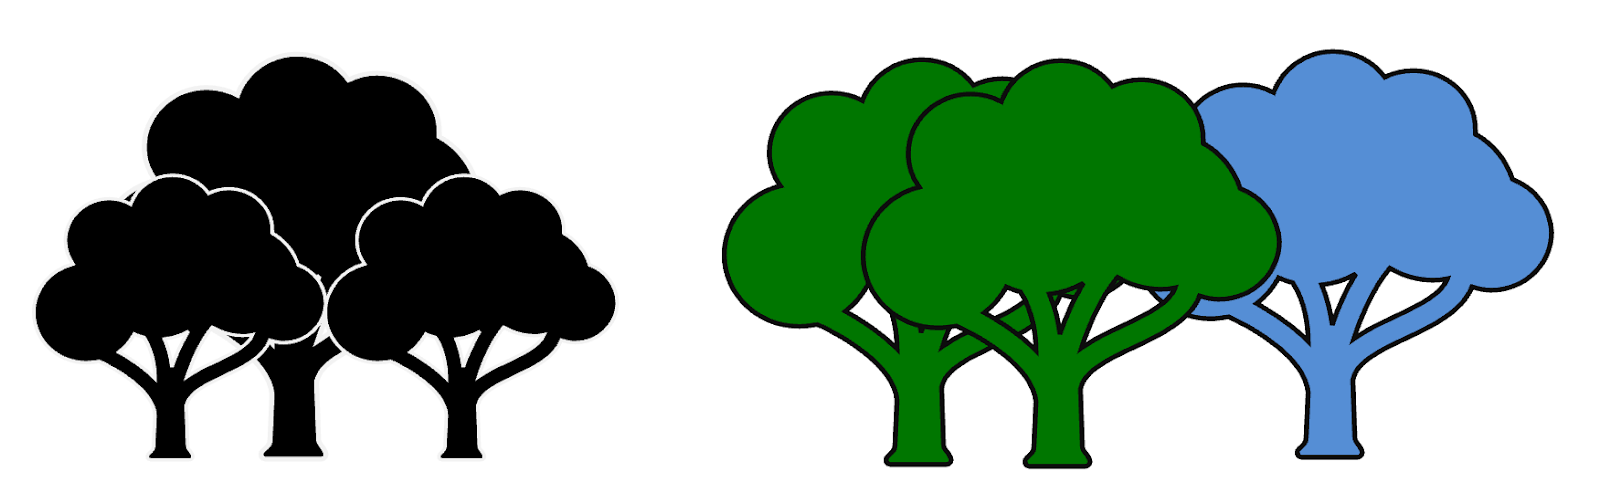
\includegraphics[width=\textwidth]{dominant_trees.png}
  \caption{Visualization of detection problems.\\ Left: a dominant tree covers subdominant
trees (challange 1).\\ Right: Close equally tall trees (green) are detected as one tree, causing
overestimation of the crown area (challange 4).}
  \label{fig:dominant_trees}
\end{figure}

\end{enumerate}
\subsection{Methodology} \label{Methodology}
% !TEX root = Master.tex

In a first step, summary statistics of the inventory data are presented to get an insight of the forest and
correlations (see Section \ref{Overview variables}).
In a second step, a regression model is constructed to estimate the diameter of trees based on the height and
crown area from the inventory data. Additionally, the effect of tree species is examined. Subsequently, the
model is used to predict the diameter of the trees in the LiDAR dataset.

\renewcommand{\labelenumi}{\arabic{enumi}.}
\begin{enumerate}

\item \textbf{The Log-normal Regression Model} \\
The log-transformation (and back-transformation) is an established method introduced in 1941 by Finney (see [4]).
The transformation of the response yields in a log-normal model 
\begin{align*}
ln(y)  =  X\beta
\end{align*}
 where $X$ is the design matrix. The
random variable 
\begin{align*}
z = ln(y)
\end{align*}
 is normally distributed with $\mu_z$ and $\sigma_z^2$. 
The back-transformed random variable 
\begin{align*}
y = e^z
\end{align*}
 is log-normal
distributed. It can be shown that 
\begin{align*}
\mu_y = e^{x_i' \beta+\sigma_z^2/2}.
\end{align*}
$\sigma_z^2$ is estimated by the MSE $s_z^2$ and $e^{\sigma_z^2}$ can be considered as a correction term, which
due to its positivity always increases the back-transformation.

\item \textbf{Generalized Linear Models} \\
Instead of transforming the response itself, Generalized Linear Models (GLM) are used to instead transform the
mean. Thus, $\mu_i$ is connected to the linear predictor
\begin{align*}
\eta_i = x'_i\beta = \beta_0 + \beta_1 x_{i1} + \beta_2 x_{i2} + ... + \beta_k x_{ik}
\end{align*}
 through 
\begin{align*}
\mu_i = h(\eta_i) = h(x'_i \beta) \quad \text{or} \quad \eta_i = g(\mu_i),
\end{align*} 
  where $h$ is the response function and $g$ the link
function [5]. The Gaussian and gamma from the exponential family are chosen. The log function
as link is chosen for the same reason as in the log-normal model. The transformation of the mean can result in
substantially different result for the Gaussian model with log link compared to the log-normal model.
The dispersion parameter 	 (see Table \ref{tab:Prediction Models}) of the Gaussian model is just the $\sigma^2$ and $v^{-1}$ (inverse scale) for the gamma
model [5].

\end{enumerate}


Bias correction is performed on compartment level, where inventory data is sparse. K-means clustering will group
compartments with similar tree structure allowing for a richer inventory set used for bias correction.

\textbf{K-means clustering} \\
K-means clustering is a relatively simple iterative clustering procedure. In short, k centroids are set randomly into the data space.


\begin{enumerate}
\renewcommand{\labelenumi}{\arabic{enumi}}
\item For each data point (compartment), the distance to the k centroids is calculated.
\item Each data point is assigned to the centroid with its minimal distance forming k-groups.
\item The mean of all data points within the group is calculated, which is essentially the update of the centroid.

\end{enumerate}


This is repeated until there is no more change of the attribution of the compartments to the clusters (convergence is
reached). As the initiation of the k-centroids is random, results can vary. The number of k-clusters must be
defined prior to the start. Different numbers of cluster k should be tested, and decision can be made by
visualization of the clusters and/or change in the total within sum squares used to pick the best (heuristic) k.
Ultimately, the clusters should make sense in a way that experts can describe them. For more details see ref. [7].\\


For each of the resulting clusters of compartnents, parametric distributions are fitted on the values of the measured and predicted tree diameter. This leads to a posession of parameters of the (chosen kind of) distribution, such that tuning of such parameters allows for bias reduction.\\

\textbf{Parametric Distribution Fitting} \\
LiDaR as well as inventory diameters on a cluster level are subject to a fit of a preselected distribution. The chosen distribution needs to be reasonable in the sense that parameter or variable restrictions are well defined and the preselected distribution should properly reflect the observed distribution [13].\\

There are several methods for fitting a parametric distribution to the data. \\
In this case, Maximum Likelihood Estimation (MLE) is applied to estimate the parameters of the distribution, i.e. the Log-Likelihood function of the respective distribution is the objective of a maximization problem with respect to the distributional parameters [15].\\

\textbf{Gamma Distribution} \\
Let X be a random variable which follows a gamma distribution: $X \sim Ga(\alpha, \beta)$, where $\alpha$ is called the shape parameter and $\beta$ is called the rate parameter.\\
The corresponding probability density function is
\begin{align*}
f(x ; \alpha , \beta) = \dfrac{\beta^\alpha x^{\alpha -1}e^{- \beta x}}{\Gamma(\alpha)}
\quad \text{for} \quad x > 0 \quad \text{and} \quad \alpha , \beta > 0,
\end{align*}
where $\Gamma(\alpha)$ is the gamma function [14].\\
\textit{"The gamma distribution is not only a good model for waiting
times, but one for many nonnegative random variables of the continuous
type. For illustrations, the distribution of certain incomes could be modelled
satisfactorily by the gamma distribution, since the two parameters $\alpha$ and $\beta$
provide a great deal of flexibility."} [14]\\

\clearpage
\section{Analysis}
% !TEX root = Master.tex

Regression models are fitted on the whole inventory dataset to predict the tree diameter distribution of the LiDAR dataset. Later, this density distribution is bias corrected on compartment level.\\

The initial problem regarding this estimation lied within the sparsity of variables.
A regression model can only use variables which exist in both datasets (LiDAR \& inventory data).\\

During the first half of this study, only the tree height and geographical position of each tree existed within the LiDAR
dataset. Further important variables were later acquired and provided by ForestEye Research GmbH \& Co. KG. An overview can be
found in Table \ref{tab:variables}.\\

Therefore, two different approaches for the regression model were developed. The regression model tackling
sparsity can be found in the Appendix, providing an alternative approach for studies which have only the height and geographical position of trees.\\

The final model is discussed in the following Sections.
\subsection{General Overview of the Variables} \label{Overview variables}
% !TEX root = Master.tex

\begin{table}[H]
\setlength\arrayrulewidth{1pt}  
\centering
\begin{adjustbox}{max width=\textwidth}
\begin{tabular}{|c|c|c|}
\hline
\rowcolor{Gray}
\textbf{Variable}    & \textbf{Data Type} & \textbf{Dataset}       \\ \hline
Diameter {[}cm{]}    & Continuous         & Inventory              \\ \hline
Crown Area {[}cm²{]} & Continuous         & LiDAR                  \\ \hline
Height {[}cm{]}      & Continuous         & LiDAR                  \\ \hline
Species (Art\_ grp)  & Factor             & LiDAR (Neural Networks) \\ \hline
\end{tabular}
\end{adjustbox}

\caption{Variables used in the study and their sources}
\label{tab:variables}
\end{table}

First the general properties of the inventory data of 2018 are examined to obtain a first intuition of dependencies
and structures for further analysis. As discussed in Section \ref{Methodology}, the diameter is predicted based on some
variables. Previous research proposed to create models individually for each tree species, using height
measurements, the crown area \& the crown area of larger trees [6].\\

Figure \ref{fig:boxplots Overview} indicates that this proposition is also valid for the measured trees in Gartow, as the boxplots of the
diameter and height differ per species. Similar patterns are seen for height and diameter,
indicating high correlation.

\begin{figure}[H]
\centering
  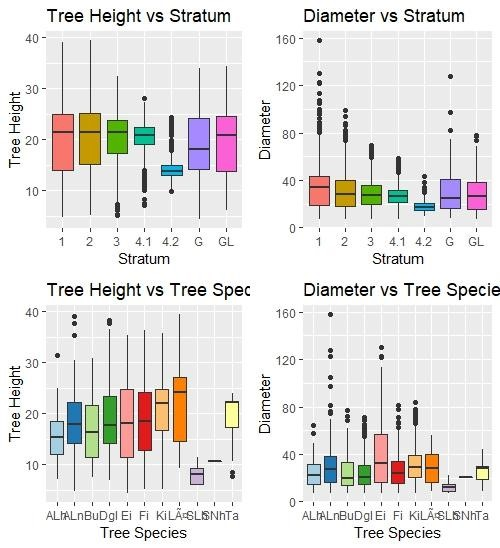
\includegraphics[scale = 0.8]{boxplots_overview.jpg}
  \caption{Boxplots based on Stratum (upper) and Tree Species (lower). Same patterns show potential correlation in height and diameter.}
  \label{fig:boxplots Overview}
\end{figure}

Figure \ref{fig:diameter vs height} underlines this expected height correlation. A strong non-linear relationship is observed. This almost
exponential curve can be explained by the natural growth of a tree. Once a tree species reaches its maximum
height, only the diameter continues to grow up to a natural limit. The effect of tree specific is well observable
comparing oaks (Ei) and pines (Ki). They are well separated between 20 and 30 meters of height.

\begin{figure}[H]
\centering
  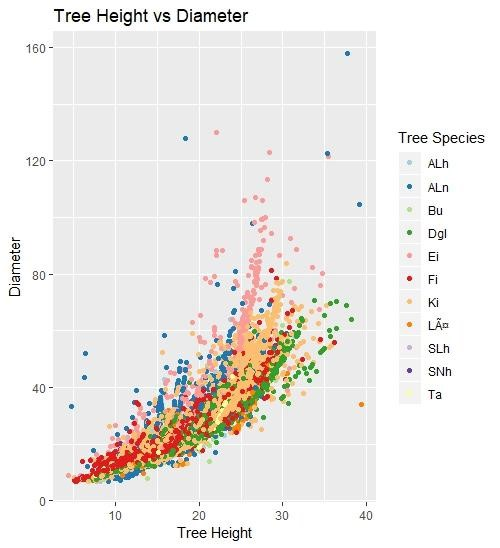
\includegraphics[scale = 0.75]{diam_vs_height.jpg}
  \caption{Relation between diameter and height. Tree species are visualized by colouring}
  \label{fig:diameter vs height}
\end{figure}

A log transformation is imposed on the response diameter (see Figure \ref{fig:log transformation diam vs height}). The log
transformation reduces the skewness of the data, while keeping a potential linear dependency. The diameter is
always positive and a log transformation can be applied. The relationship between height and log(diameter) has
improved regarding linearity.

\begin{figure}[H]
\centering
  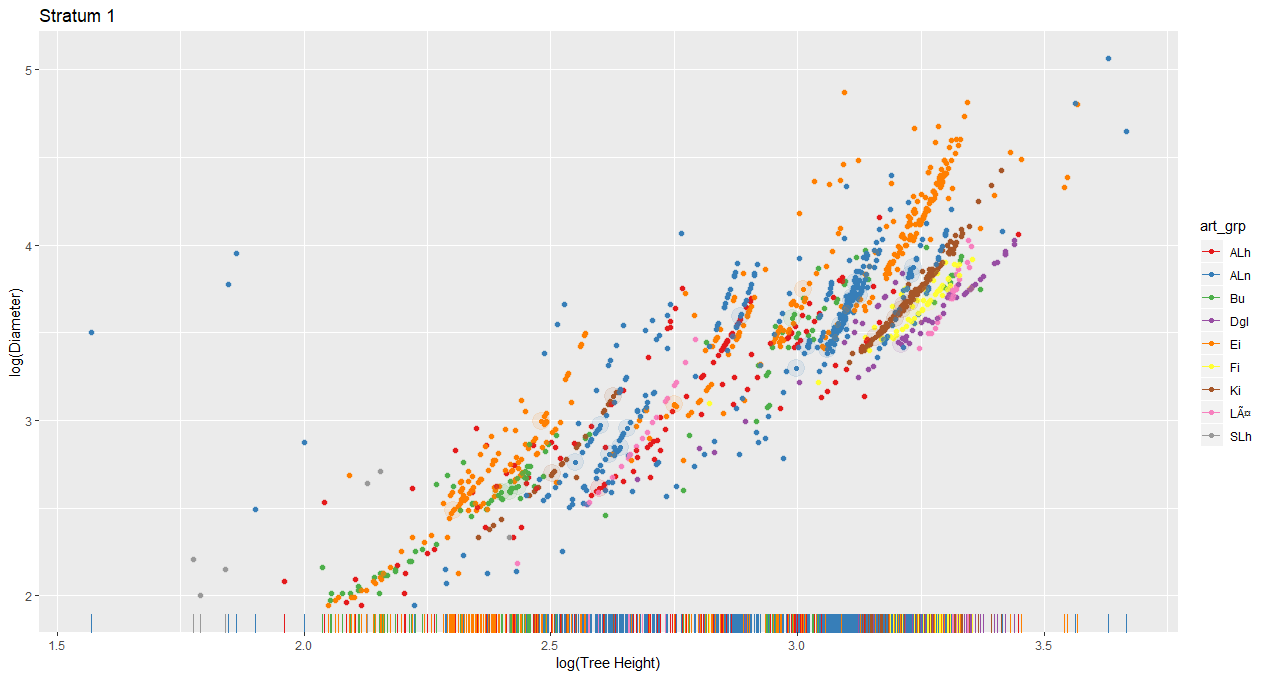
\includegraphics[scale = 0.45]{log_diam_vs_height.png}
  \caption{Scatterplot of log transformed diameter and height for Stratum 1.}
  \label{fig:log transformation diam vs height}
\end{figure}



\subsection{Regression Models} \label{Regression Models}
% !TEX root = Master.tex

To predict the diameter of a tree using regression models is straight forward. We chose the later described regression models based on following criteria. \\

\renewcommand{\labelenumi}{\arabic{enumi}.}
\begin{enumerate}

\item \textit{Interpretability} is required so experts can understand the results to continue to work with the proposed models. Inference on all covariates must be feasible, as large standard errors (i.e. high uncertainty in the predicted diameter) causes the model to be unusable.

\item \textit{Generalization} (i.e. the goodness of fit to new data) must be high to assure sufficient prediction of the diameter
of trees detected by LiDAR. While it is likely that regression splines might result in an overall better fit to the data,
relying too much on the sampling data might cause substantial over-fitting. As described in Section \ref{Challenges},
over-fitting must be prevented due to the unreliability in the data. Regularization methods such as ridge
regression could be applied. Yet, based on the results in the applied models it was not further investigated.

\item \textit{Complexity} should be kept moderate to again make the models more accessible. The model is only used in
this study to predict the diameter. Using Generalized Additive Models for Location Scale and Shape could be an
interesting addition to this study to further investigate the uncertainty at different in the estimates but is potentially too
complex for the task of a simple prediction.

\end{enumerate}

Based on those criteria, a log-linear model (based on the observations in Section \ref{Overview variables}) and generalized linear models are
compared.
\subsection{The Regression Outputs} \label{Regression Outputs}
% !TEX root = Master.tex


All regression models are fitted using all available covariates: 
\begin{align*}
\text{Diameter} \sim \text{Tree Height} + \text{Crown Area} + \text{factor(Species)}
\end{align*}

\begin{table}[H]
\setlength\arrayrulewidth{1pt}
\centering

\begin{adjustbox}{max width=\textwidth}
\begin{tabular}{|c| c c| c c| c c|}
\hline
\rowcolor{SeaBlue}
 \multicolumn{1}{|c|}{\textbf{Coefficients}} &  \multicolumn{2}{|c|}{\textbf{Log-linear Model}} &  \multicolumn{2}{|c|}{\textbf{GLM Gaussian (Link: Log)}} &  \multicolumn{2}{|c|}{\textbf{GLM gamma (Link: Log)}}  \\
\hline 
\rowcolor{Gray}
\multicolumn{1}{|c|}{-} & \multicolumn{2}{|c|}{Estimate \& Std. Error} & \multicolumn{2}{|c|}{Estimate \& Std. Error} & \multicolumn{2}{|c|}{Estimate \& Std.Error} \\ 
\hline 
Intercept & 1.685 & 0.010 & 1.498 & 0.014 & 1.709 & 0.010 \\ 
\hline 
Height & 0.081 & 0.000 & 0.091 & 0.001 & 0.081 & 0.000 \\ 
\hline 
Crown Area & 0.001 & 0.000 & 0.001 & 0.000 & 0.001 & 0.000 \\ 
\hline 
Art\_ grpDgl & -0.296 & 0.008 & -0.415 & 0.008 & -0.305 & 0.008 \\ 
\hline 
Art\_ grpEi & 0.183 & 0.010 & 0.222 & 0.008 & 0.174 & 0.010 \\ 
\hline 
Art\_ grpFi & -0.185 & 0.009 & -0.259 & 0.009 & -0.195 & 0.009 \\ 
\hline 
Art\_ grpKi & -0.115 & 0.007 & -0.139 & 0.007 & -0.125 & 0.007 \\ 
\hline 
Art\_ grpLä & -0.250 & 0.015 & -0.323 & 0.015 & -0.254 & 0.016 \\ 
\hline 
Overdispersion $\Phi$ & - & - & 12.5 & - & 0.01 & - \\ 
\hline 
\end{tabular} 
\end{adjustbox}

\caption{Diameter prediction models: log-linear, Gaussian and gamma}
\label{tab:Prediction Models}

\end{table}

The estimates in all models (see Table \ref{tab:Prediction Models}) are significantly different from 0. The untransformed confidence
intervals are visualized in Figure \ref{fig:Coefficients}. The transformed confidence intervals for the gamma model are found in
Table \ref{tab:CI}.

\begin{figure}[H]
  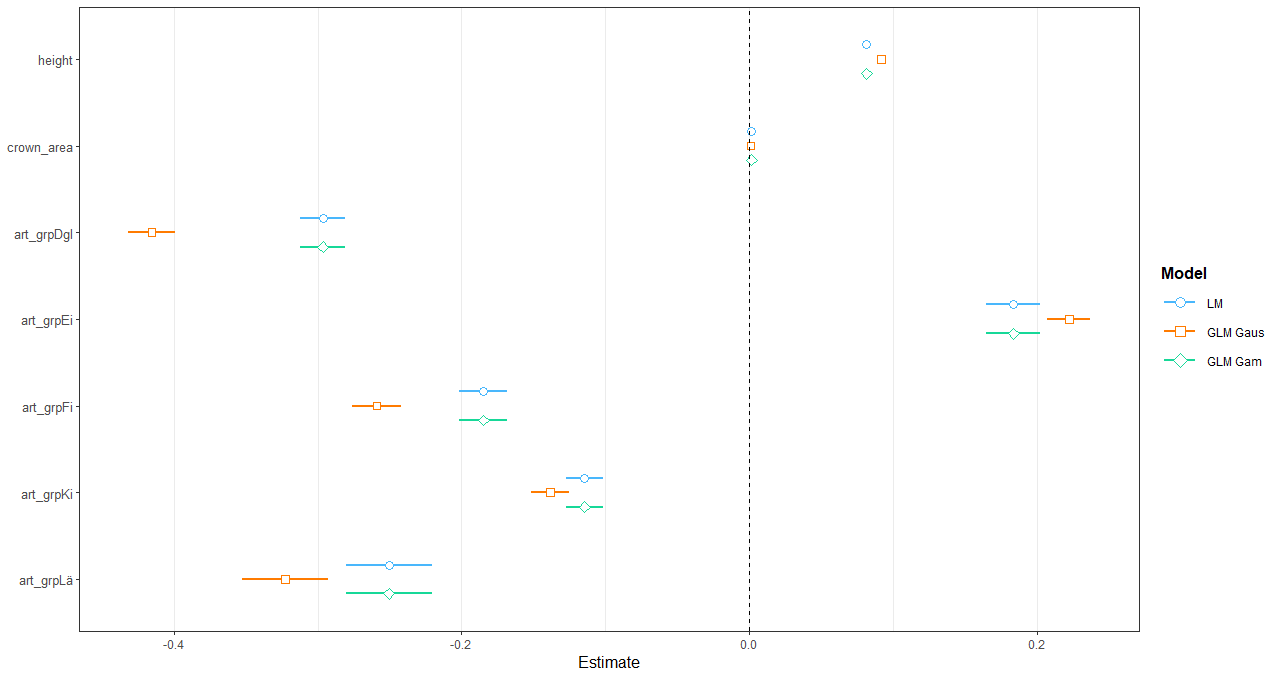
\includegraphics[width=\textwidth]{figures/coefficients.png}
  \caption{While the estimates and confidence intervals of the gamma and log-linear model tend to be similar. The Gaussian model estimates are larger for values greater 0 and smaller for values smaller then 0.}
  \label{fig:Coefficients}
\end{figure}


\begin{table}[H]
\setlength\arrayrulewidth{1pt}
\centering
\begin{adjustbox}{max width=\textwidth}
\begin{tabular}{|c| c| c| c|}
\hline 
\rowcolor{Gray}
\textbf{Coefficient} & \textbf{2.5\% CI Lower bound} & \textbf{97.5\% CI Upper bound} & \textbf{CI Width} \\
\hline
Intercept & 5.4170 & 5.6320 & 0.2150 \\ 
\hline 
Height & 1.0831 & 1.0851 & 0.0020 \\ 
\hline 
Crown Area & 1.0013 & 1.0016 & 0.0003 \\ 
\hline 
Art\_ grpDgl & 0.7250 & 0.7488 & 0.0238 \\ 
\hline 
Art\_ grpEi & 1.1666 & 1.2135 & 0.0469 \\ 
\hline 
Art\_ grpFi & 0.8085 & 0.8375 & 0.0290 \\ 
\hline 
Art\_ grpKi & 0.8704 & 0.8943 & 0.0239 \\ 
\hline 
Art\_ grpLä & 0.7515 & 0.8002 & 0.0487 \\ 
\hline 
\end{tabular} 
\end{adjustbox}

\caption{Transformed confidence intervals (CI) and width of the gamma model in cm}
\label{tab:CI}


\end{table}

Model selection is done by three criterions: R² , AIC \& BIC and Residual Sum of Squares (RSS)
\begin{align*}
\sum{(y - \hat{y_{predict}})^2}.
\end{align*}
\\
All values can be found in Table \ref{Model Selection}.


\begin{table}[H]
\setlength\arrayrulewidth{1pt}
\centering
\begin{adjustbox}{max width=\textwidth}
\begin{tabular}{|c|c|c|c|c|c|}
\hline
\rowcolor{Gray}
\textbf{-}                                                                               & \textbf{LM}       & \multicolumn{2}{c|}{\textbf{GLM Gaussian}} & \multicolumn{2}{c|}{\textbf{GLM gamma}} \\ \hline
\multirow{3}{*}{\begin{tabular}[c]{@{}c@{}}R² / Pseudo R² \\ (Cragg-Uhler)\end{tabular}} & \multirow{2}{*}{} & Null Deviance             & 654900         & Null Deviance            & 533.9        \\ \cline{3-6} 
                                                                                         &                   & Residual Deviance         & 46260          & Residual Deviance        & 35.72        \\ \cline{2-6} 
                                                                                         & 0.937             & \multicolumn{2}{c|}{0.929}                 & \multicolumn{2}{c|}{0.933}              \\ \hline
AIC                                                                                      & -                 & \multicolumn{2}{c|}{19903.18}              & \multicolumn{2}{c|}{19102.88}           \\ \hline
BIC                                                                                      & -                 & \multicolumn{2}{c|}{19959.15}              & \multicolumn{2}{c|}{19158.84}           \\ \hline
RSS                                                                                      & 60136.49          & \multicolumn{2}{c|}{46257.25}              & \multicolumn{2}{c|}{53569.47}           \\ \hline
RSE ($\sqrt{RSS/n}$)                                                                                  & 4.0315            & \multicolumn{2}{c|}{3.53581}               & \multicolumn{2}{c|}{3.80503}            \\ \hline
\end{tabular}
\end{adjustbox}

\caption{Model selection criterion for Log-linear, Gaussian and gamma}
\label{Model Selection}
\end{table}

The models have a (pseudo) R² of almost 93\% while the Log-linear model is favorable with 93.7\% explained variation. The AIC \& BIC of the gamma model is better compared to the Gaussian model. This cannot be compared to the Linear Model, of which the AIC is constructed based on the RSS and not a likelihood. Finally, the Gaussian model has the lowest Sum Squares and therefore the smallest Residual Standard Error with approximately 3.53 cm in the diameter.\\

All models have an exceptional fit, whereby we finally decide to use the gamma model. A bias correction
is introduced by fitting parametric distributions in Section \ref{Distribution Engineering}. Thus, the model with the highest likelihood (AIC \& BIC) is finally favoured.\\

Figure \ref{fig:Pane} visualizes the good fit of the model. Most points by species are well described by the panes, whereby
we see for both tree species an underestimation at large value. This is expected, as trees have natural high
limits. Once it is reached, only the diameter increases, resulting in the underestimation. \\

\begin{figure}[H]
  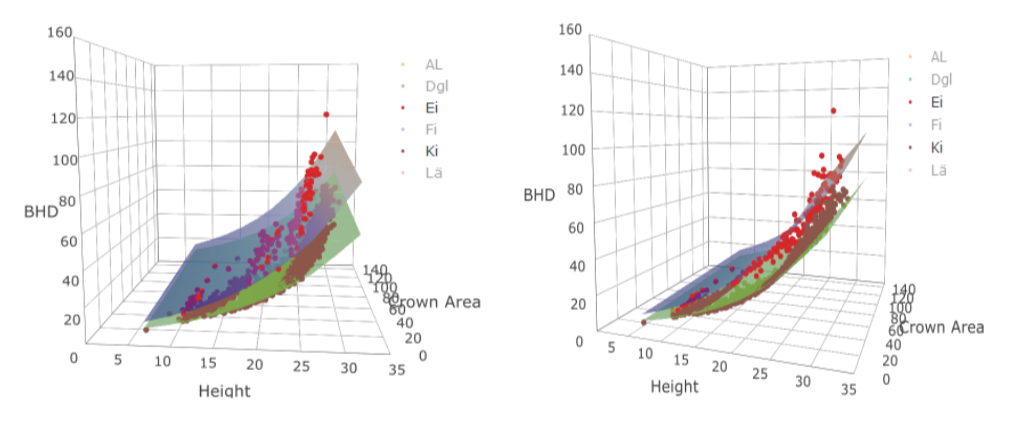
\includegraphics[width=\textwidth]{predicted_pane.png}
  \caption{Predicted pane of the gamma model for oaks (Ei red) and pines (Ki brown)}
  \label{fig:Pane}
\end{figure}

Figure \ref{fig:Residuals GLM gamma} displays the residual plots of the gamma model. Some unwanted behavior is seen in the scale location
plot, which is used to identify violations of homoscedasticity. A somewhat linear behavior between 2.5 to 3
followed by a curvature to 4 results in potential mild heteroskedasticity for larger values as indicated by the red
line. 5 unique observations in over 3700 observations
are identified as outliers. This leads to the conclusion that the GLM gamma fits well and is acceptable regarding
the underlying assumptions.

\begin{figure}[H]
  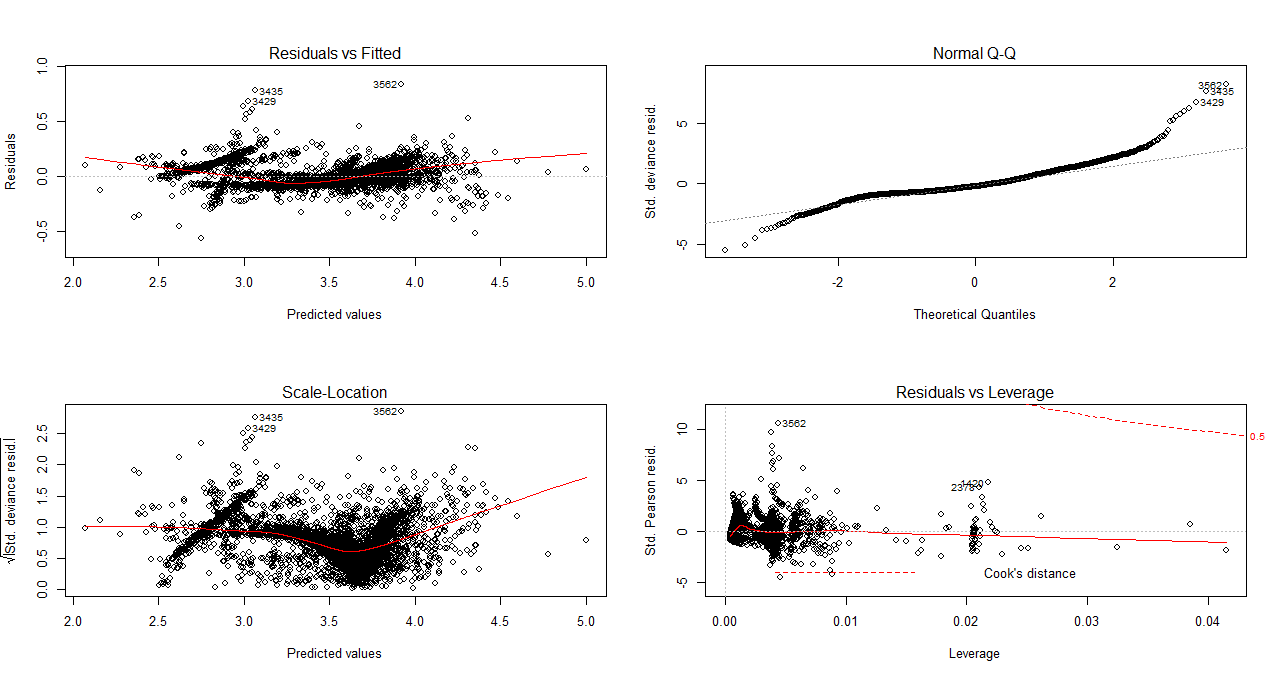
\includegraphics[width=\textwidth]{residuals_glm_gamma.png}
  \caption{Residual plots of GLM gamma. Data points with an index are considered outliers.}
  \label{fig:Residuals GLM gamma}
\end{figure}

\subsection{Clustering} \label{Clustering}
% !TEX root = Master.tex

A crucial part of this study is the cluster analysis of the forest compartments. Therefore, we perform simple k-means clustering on the compartments to resolve a key issue: The single compartments themselves do not have enough
observations to perform any kind of distribution fitting via Maximum Likelihood Estimation. Clustering relatively similar compartments could resolve
this issue by creating k clusters, whereby each cluster then has enough observations to perform distribution fitting.\\

The following auxiliary variables are assigned to each of the compartments to calculate distances. The thought process of those variables to describe the systematic bias is further outlined in Table \ref{tab:auxiliary_variables}.

\begin{table}[H]
\setlength\arrayrulewidth{1pt}
\centering
\begin{adjustbox}{max width=\textwidth}
\begin{tabular}{|c|c|}
\hline
\rowcolor{Gray}
\textbf{Variable}                                                                              & \textbf{Potential to explain Bias}                                                                                                                                   \\ \hline
\begin{tabular}[c]{@{}c@{}}Forest Cover Ratio\\ Area / \# of Detected Trees\end{tabular}       & \multirow{2}{*}{\begin{tabular}[c]{@{}c@{}}A densely forested region will have more dominant\\ subdominant structures.\end{tabular}}                                 \\ \cline{1-1}
\begin{tabular}[c]{@{}c@{}}Tree crown coverage\\ Area surface  - Total Crown Area\end{tabular} &                                                                                                                                                                      \\ \hline
Variation of crown area                                                                        & \multirow{2}{*}{\begin{tabular}[c]{@{}c@{}}Large variation in the Tree Crowns and overall large crowns\\ will have more dominant subdominant structure\end{tabular}} \\ \cline{1-1}
0.75 quantile of crown area                                                                    &                                                                                                                                                                      \\ \hline
Variation of height                                                                            & \begin{tabular}[c]{@{}c@{}}If the cultivation time is similar, the trees should be of same\\ height, resulting in less covering\end{tabular}                         \\ \hline
\end{tabular}
\end{adjustbox}

\caption{Auxiliary variables for k-mean clustering}
\label{tab:auxiliary_variables}
\end{table}

All variable combinations were tested by a time-consuming trial-and-error procedure. Meaning that for each
generated cluster output, a Principle Component Analysis is performed (if > 2 variables), visualizing the goodness
of separation from each group (Figure \ref{fig:Clusterplot}). Subsequently 3-D plots from the LiDAR dataset for
several compartments of each cluster are created. Clustering is considered successful, once the groups can be well
explained by the 3-D images and the separation of the clusters is reasonable.\\
This is presented with the final model used in this study.\\

\begin{figure}[H]
\centering
  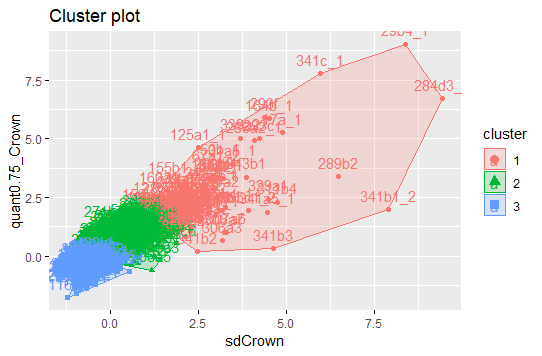
\includegraphics[scale = 0.85]{clusterplot.png}
  \caption{Scatterplot of the sections with the grouping based on k-means clustering}
  \label{fig:Clusterplot}
\end{figure}

The chosen final auxiliary variables are the 0.75 quantile of the crown area and the variation of the crown area.
Figure \ref{fig:Clusterplot} shows high correlation. This is additionally depicted in Figure \ref{fig:Boxplots Cluster}. The desired property of a clear separation of the clusters is not fully given. We render this as a
minor problem. The three cluster are large enough so that enough samples from inventory data are in each
cluster. Cluster 1 336, cluster 2 4180, cluster 3 5471.\\

\begin{figure}[H]
\centering
  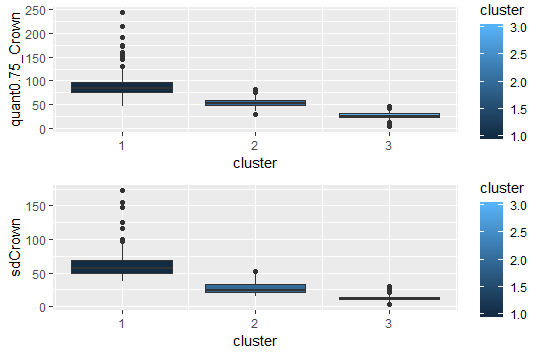
\includegraphics[scale = 0.85]{boxplots_cluster.png}
  \caption{Boxplots for the used variables - clusters}
  \label{fig:Boxplots Cluster}
\end{figure}


The 3-D plots of some compartments for each cluster offer insights into the goodness of the clustering. Sections in
cluster 1 appear to be very dense areas as the forests soil is barely visible. Interestingly, the tree height appears
to be rather equal, resulting in homogeneous patches. This is well depicted by compartment 261a2 (Figure \ref{fig:LiDAR Cluster 1}). The
compartment in cluster 2 are sparser wooded (Figure \ref{fig:LiDAR Cluster 2}). Blue patches (forest soil) are visible in every compartment. This is even
stronger pronounced in the compartments of cluster 3 (Figure \ref{fig:LiDAR Cluster 3}).


\begin{figure}[H]
  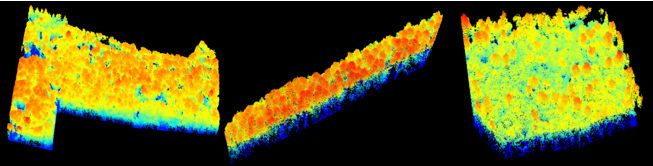
\includegraphics[width=\textwidth]{cluster1_lidar.png}
  \caption{Cluster 1 section ID's from left to right: 155a1, 311b1, 261a2}
  \label{fig:LiDAR Cluster 1}
\end{figure}

\begin{figure}[H]
  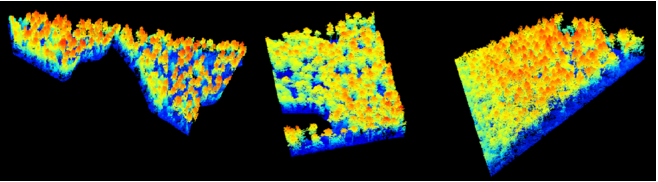
\includegraphics[width=\textwidth]{cluster2_lidar.png}
  \caption{Cluster 2 section ID's from left to right: 37a2, 71b5, 309a2}
  \label{fig:LiDAR Cluster 2}
\end{figure}

\begin{figure}[H]
  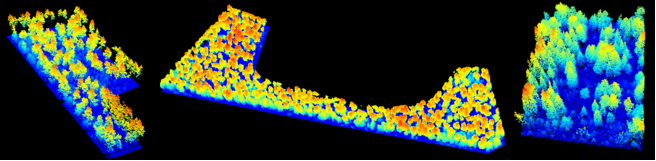
\includegraphics[width=\textwidth]{cluster3_lidar.png}
  \caption{ Cluster 3 section IDs from left to right: 314a2, 207a2, 36c1}
  \label{fig:LiDAR Cluster 3}
\end{figure}

Using the variable tree crown to describe the clusters is difficult. No actual difference in the variation and quantile
of the crown area between the clusters can be observed visually. Anyhow, dense and sparse
forested region are well separated.\\

It might be explained as following. Dense compartments show regions of equally height trees. The tree detection
algorithm is unable to detect all trees, as tree crowns of several trees are detected as one (see Section \ref{Challenges}). This
leads to unnatural high variation in the crown area. The quantile of the crown area further captures the extent of
this effect.


\subsection{Distribution Engineering} \label{Distribution Engineering}
% !TEX root = Master.tex

After predicting the tree diameter of the LiDAR data, a systematic bias occurs due to the downsides of the LiDAR system difficulties mentioned in Section \ref{Challenges}. To overcome such kind of obstacles of the main goal, i.e. approximating an ideally unbiased diameter distribution of the forest on a compartment level, we introduced a technique which they refer to as "distribution engineering". It takes advantage of some features and diagnostics of parametric distributions. The usefulness of the clusters is also presented in this Section.\\

\begin{figure}[H]
\centering
  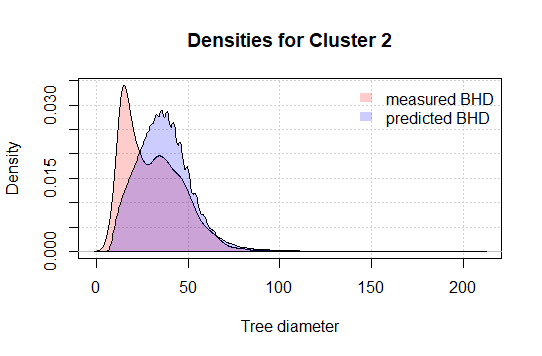
\includegraphics[scale = 0.8]{dens2.png}
  \caption{Measured vs predicted densities of the tree diameter for compartments of the $2^{nd}$ cluster}
  \label{fig:example_dens2}
\end{figure}


In a first step, the diameter values of the LiDAR data as well as the inventory data are subject to a parametric distribution fit. This initial fit is employed on a cluster level, which provides us with the respective parameters of those distributions. In particular but not exclusively, a gamma distribution is fitted in this case (using R-Package: fitdistrplus [16]). The reasoning behind that is to retain coherence, since a GLM gamma regression model was applied to predict the tree diameter. An example for cluster 2 with further details of the fits can be observed in Figure \ref{fig:Fits}.

\begin{figure}[H]
\centering
\begin{subfigure}{.5\textwidth}
  \centering
  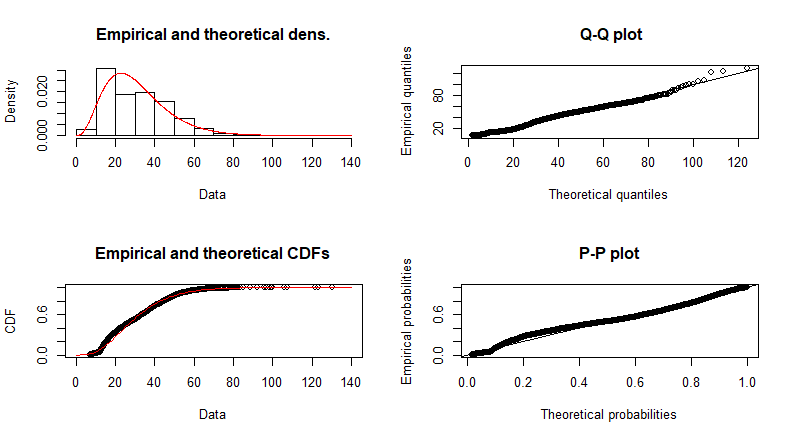
\includegraphics[width=.9\linewidth]{cluster2_valid.png}
  \caption{Inventory}
  \label{fig:cluster2_valid}
\end{subfigure}%
\begin{subfigure}{.5\textwidth}
  \centering
  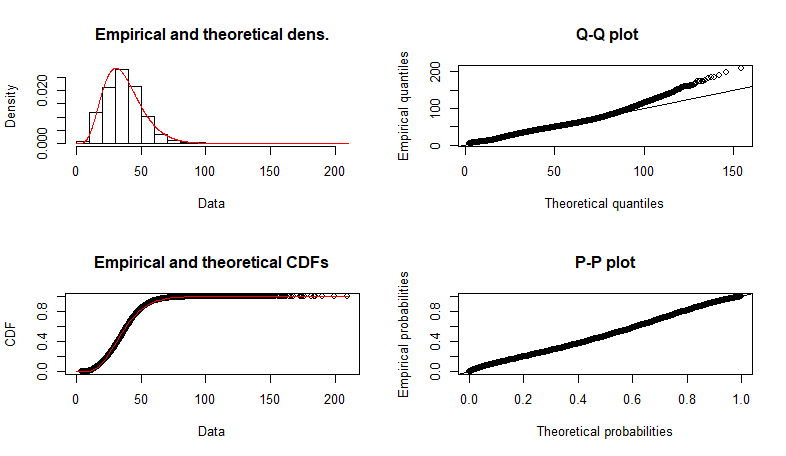
\includegraphics[width=0.85\linewidth]{cluster2_pred.png}
  \caption{LiDAR}
  \label{fig:cluster2_pred}
\end{subfigure}
\caption{Graphical fit diagnostics for cluster 2 - Tree diameter}
\label{fig:Fits}
\end{figure}

Looking at the QQ-Plot of Figure \ref{fig:cluster2_pred}, one can clearly see the outliers of the predicted tree diameter on the upper quanitles (LiDAR), which is (amongst other things) attributed to the overestimation of the crown area discussed previously in Sections \ref{Challenges} \& \ref{Clustering}.\\

The density function of a gamma distribution is composed of a function containing two parameters, the shape parameter $\alpha_{i,j}$ and the rate parameter $\beta_{i,j}$, where $i$ is the cluster index and 
$j$ indicates the data source (Inventory or LiDAR). \\

A summary of the distribution fits can be found in Tables \ref{tab:fitdistrplus_inventory} - \ref{tab:fitdistrplus_lidar}.

\begin{table}[H]
\setlength\arrayrulewidth{1pt}  
\centering
\begin{adjustbox}{max width=\textwidth}
\begin{tabular}{|c|c|c|c|c|c|}
\hline
\rowcolor{Gray}
\textbf{Cluster} & \textbf{Shape} & \textbf{Rate} & \textbf{Log-Likelihood} & \textbf{AIC} & \textbf{BIC} \\ \hline
1                & 6.012          & 0.225        & -20512.63               & 41029.25     & 41042.47     \\ \hline
2                & 3.234          & 0.238         & -1498.457               & 3000.914     & 3008.548     \\ \hline
3                & 3.810          & 0.124         & -17076.31               & 34156.61     & 34169.29     \\ \hline
\end{tabular}
\end{adjustbox}
\caption{Summary of gamma distribution fit on tree diameter of inventory data by MLE}
\label{tab:fitdistrplus_inventory}
\end{table}


\begin{table}[H]
\setlength\arrayrulewidth{1pt}  
\centering
\begin{adjustbox}{max width=\textwidth}
\begin{tabular}{|c|c|c|c|c|c|}
\hline
\rowcolor{Gray}
\textbf{Cluster} & \textbf{Shape} & \textbf{Rate} & \textbf{Log-Likelihood} & \textbf{AIC} & \textbf{BIC} \\ \hline
1                & 9.013          & 0.380         & -4844594                & 9689191      & 9689216      \\ \hline
2                & 4.595          & 0.109         & -122176.7               & 244357.3     & 244373.8     \\ \hline
3                & 5.925          & 0.161         & -17076.31               & 2880304      & 2880325      \\ \hline
\end{tabular}
\end{adjustbox}
\caption{Summary of gamma distribution fit on predicted tree diameter of LiDAR data by MLE}
\label{tab:fitdistrplus_lidar}
\end{table}



This leads to the second step of this procedure, i.e. calculating the correction terms
\begin{align*}
 c_{\alpha_i} = \dfrac{\alpha_{i,invent}}{\alpha_{i,lidar}} \quad \text{and} \quad c_{\beta_i} = \dfrac{\beta_{i,invent}}{\beta_{i,lidar}}
\end{align*}
for every cluster $i$.\\

By multiplying the correction terms with the respective shape and rate parameters of the LiDAR based fit, we obtain the new (corrected) parameters:
\begin{align*}
\alpha^*_i = c_{\alpha_i} * \alpha_{i,lidar} \quad \text{and} \quad \beta^*_i = c_{\beta_i} * \beta_{i,lidar}
\end{align*}
\\

To demonstrate that the corrected parameters return a new and significantly less biased distribution as we would expect, Figures \ref{fig:cluster1_entire_corrected} - \ref{fig:cluster3_entire_corrected} are depicted to compare the old and new densities of the LiDAR diameters with respect to the diameter densities of the inventory. It shall be emphasized that the densities from the inventory data serve as a reference for how the actual densities may look like.

\begin{figure}[H]
\centering
\begin{subfigure}{.5\textwidth}
  \centering
  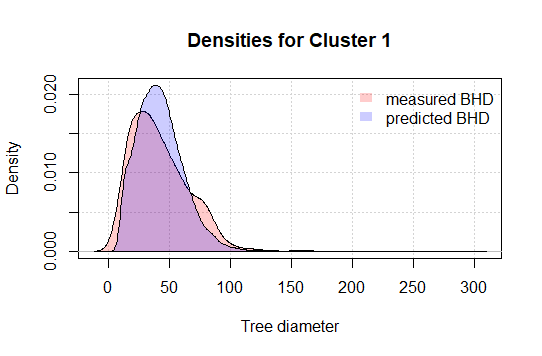
\includegraphics[width=.9\linewidth]{dens1.png}
  \caption{Densities before applying correction terms}
  \label{fig:dens1}
\end{subfigure}%
\begin{subfigure}{.5\textwidth}
  \centering
  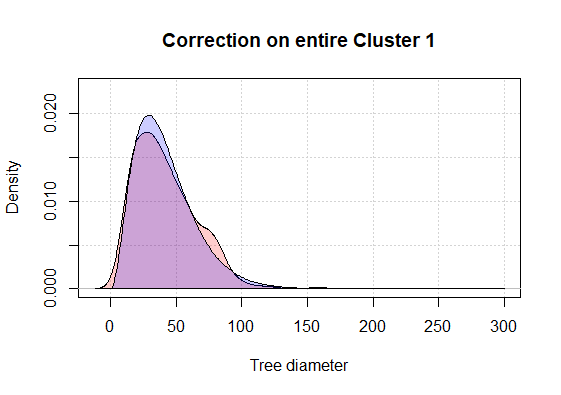
\includegraphics[width=0.843\linewidth]{correction_entire_cluster1.png}
  \caption{Densities after applying correction terms}
  \label{fig:cluster1_pred}
\end{subfigure}
\caption{Measured vs predicted densities of the tree diameter for the $1^{st}$ cluster - Comparison}
\label{fig:cluster1_entire_corrected}
\end{figure}

\begin{figure}[H]
\centering
\begin{subfigure}{.5\textwidth}
  \centering
  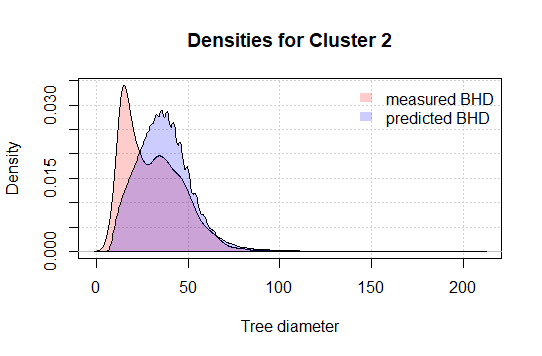
\includegraphics[width=.9\linewidth]{dens2.png}
  \caption{Densities before applying correction terms}
  \label{fig:dens2}
\end{subfigure}%
\begin{subfigure}{.5\textwidth}
  \centering
  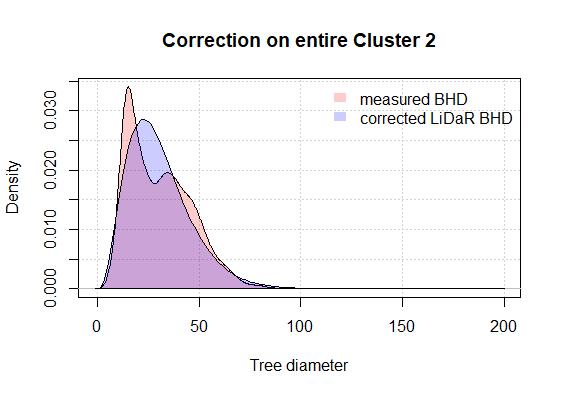
\includegraphics[width=0.845\linewidth]{correction_entire_cluster2.png}
  \caption{Densities after applying correction terms}
  \label{fig:cluster2_pred}
\end{subfigure}
\caption{Measured vs predicted densities of the tree diameter for the $2^{nd}$ cluster - Comparison}
\label{fig:cluster2_entire_corrected}
\end{figure}

\begin{figure}[H]
\centering
\begin{subfigure}{.5\textwidth}
  \centering
  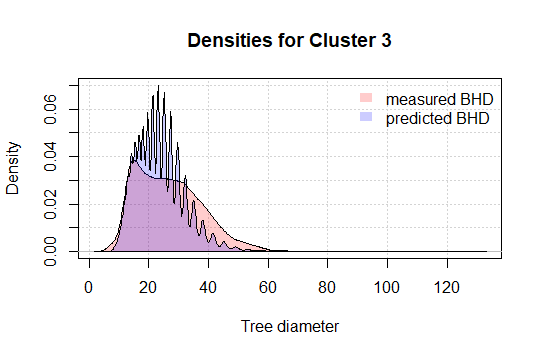
\includegraphics[width=.9\linewidth]{dens3.png}
  \caption{Densities before applying correction terms}
  \label{fig:dens3}
\end{subfigure}%
\begin{subfigure}{.5\textwidth}
  \centering
  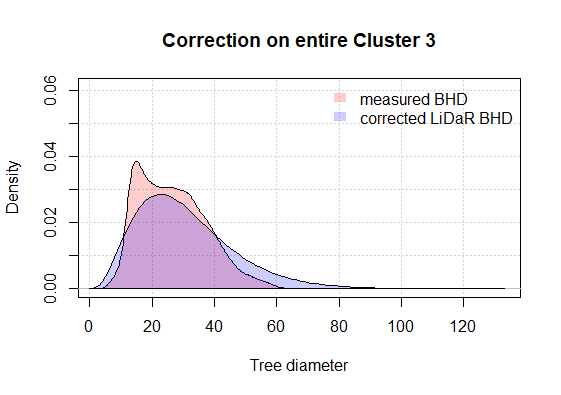
\includegraphics[width=0.842\linewidth]{correction_entire_cluster3.png}
  \caption{Densities after applying correction terms}
  \label{fig:cluster3_pred}
\end{subfigure}
\caption{Measured vs predicted densities of the tree diameter for the $3^{rd}$ cluster - Comparison}
\label{fig:cluster3_entire_corrected}
\end{figure}

Nevertheless, the aim of this technique is to reduce bias on a lower hierarchical level, namely the compartments. Therefore, for every single compartment a gamma distribution is obtained with (corrected) shape and rate parameters 
\begin{align*}
\alpha_{i,k}^* = c_{\alpha_i} * \alpha_{i,k} \quad \text{and} \quad \beta_{i,k}^* = c_{\beta_i} * \beta_{i,k},
\end{align*}
 where $i$ is the cluster allocation of compartment $k$, $\alpha_{i,k}$ and $\beta_{i,k}$ are the shape and rate parameters of the LiDAR based fit on compartment $k$.\\
  Some examples can be seen in Figures \ref{fig:correction_polygon_218a} - \ref{fig:correction_polygon_140a}.

% 218a
\begin{figure}[H]
\centering
\begin{subfigure}{.5\textwidth}
  \centering
  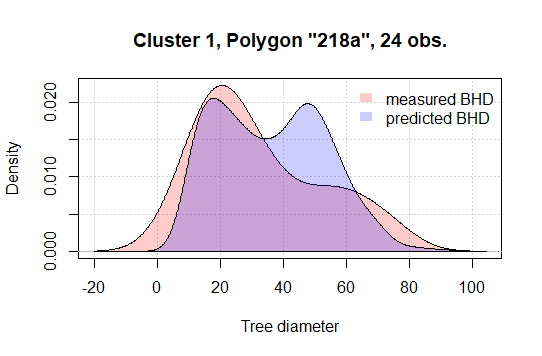
\includegraphics[width=.9\linewidth]{cluster1_218a_24.png}
  \caption{Densities before applying correction terms}
  \label{fig:polygon_before_218a}
\end{subfigure}%
\begin{subfigure}{.5\textwidth}
  \centering
  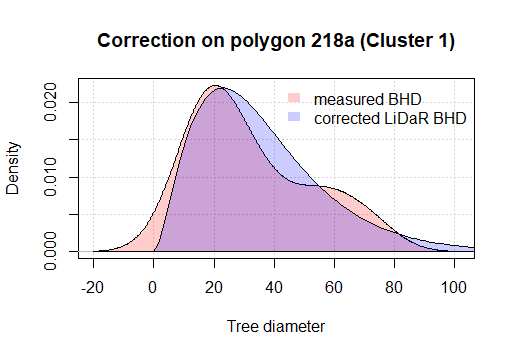
\includegraphics[width=0.86\linewidth]{corrected_cluster1_218a.png}
  \caption{Densities after applying correction terms}
  \label{fig:polygon_after_218a}
\end{subfigure}
\caption{Measured vs predicted densities of the tree diameter for compartment 218a}
\label{fig:correction_polygon_218a}
\end{figure}

% 295a1
\begin{figure}[H]
\centering
\begin{subfigure}{.5\textwidth}
  \centering
  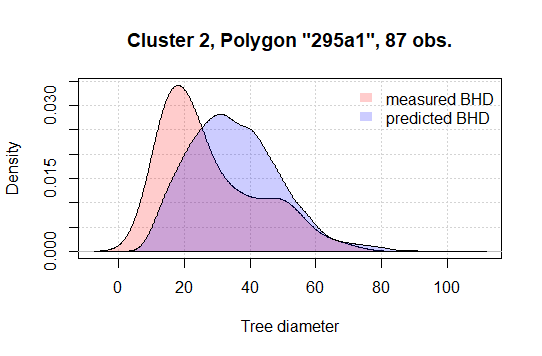
\includegraphics[width=.9\linewidth]{cluster2_295a1_87.png}
  \caption{Densities before applying correction terms}
  \label{fig:polygon_before_295a1}
\end{subfigure}%
\begin{subfigure}{.5\textwidth}
  \centering
  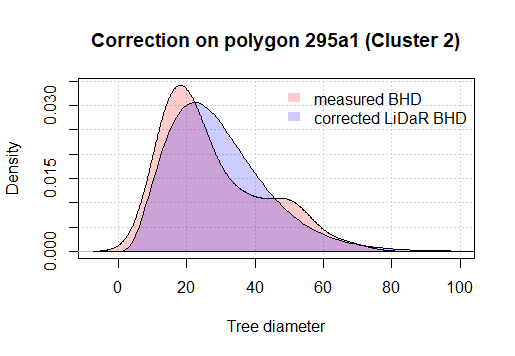
\includegraphics[width=0.853\linewidth]{corrected_cluster2_295a1.png}
  \caption{Densities after applying correction terms}
  \label{fig:polygon_after_295a1}
\end{subfigure}
\caption{Measured vs predicted densities of the tree diameter for compartment 295a1}
\label{fig:correction_polygon_295a1}
\end{figure}

% 275a2
\begin{figure}[H]
\centering
\begin{subfigure}{.5\textwidth}
  \centering
  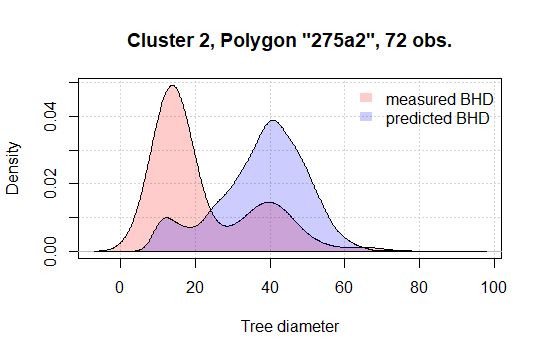
\includegraphics[width=.9\linewidth]{cluster2_275a2_72.png}
  \caption{Densities before applying correction terms}
  \label{fig:polygon_before_275a2}
\end{subfigure}%
\begin{subfigure}{.5\textwidth}
  \centering
  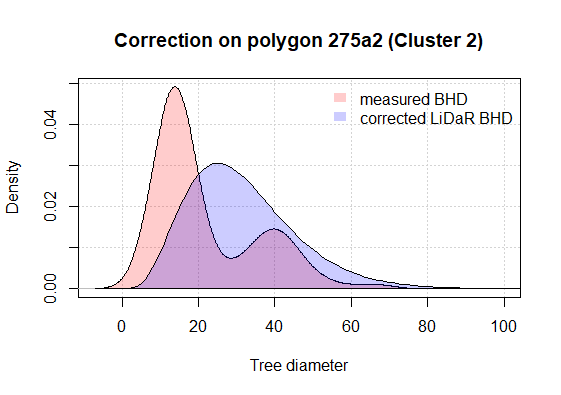
\includegraphics[width=0.837\linewidth]{corrected_cluster2_275a2.png}
  \caption{Densities after applying correction terms}
  \label{fig:polygon_after_275a2}
\end{subfigure}
\caption{Measured vs predicted densities of the tree diameter for compartment 275a2}
\label{fig:correction_polygon_275a2}
\end{figure}

% 140a
\begin{figure}[H]
\centering
\begin{subfigure}{.5\textwidth}
  \centering
  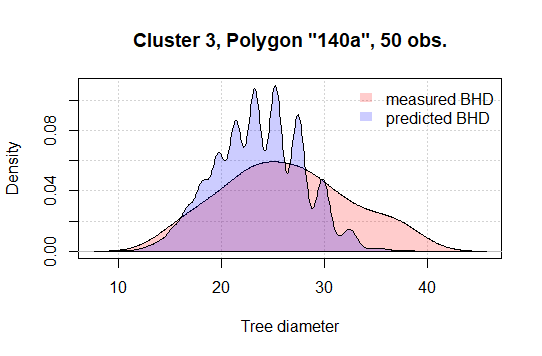
\includegraphics[width=.9\linewidth]{cluster3_140a_50.png}
  \caption{Densities before applying correction terms}
  \label{fig:polygon_before_140a}
\end{subfigure}%
\begin{subfigure}{.5\textwidth}
  \centering
  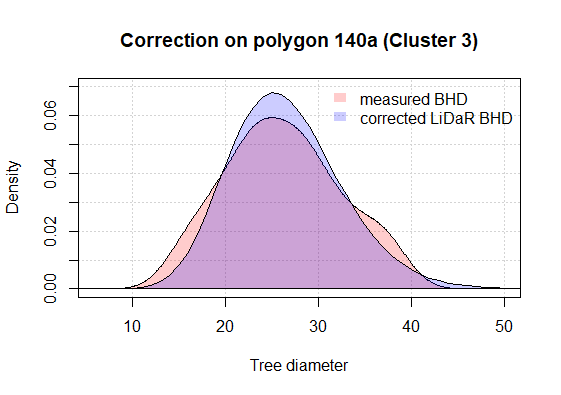
\includegraphics[width=0.835\linewidth]{corrected_cluster3_140a.png}
  \caption{Densities after applying correction terms}
  \label{fig:polygon_after_140a}
\end{subfigure}
\caption{Measured vs predicted densities of the tree diameter for compartment 140a}
\label{fig:correction_polygon_140a}
\end{figure}

Advantageously, corrected diameter densities from LiDAR data can be estimated even if there was no sampling carried out on a specific compartment. All that is needed is the compartment's allocation to a certain cluster. Another resolved issue using this method is that the corrected densities do no longer show long tails, meaning that overestimation is dealt with efficiently.
\subsection{Validation of the Results} \label{Results}
% !TEX root = Master.tex

The methodology is validated by comparing the predicted mean diameter to the mean diameter from the inventory data on compartment level. Figure \ref{fig:radius} depicts the results, whereby the predicted mean radius is obtained by sampling 1000
diameters from the corrected density distribution of the appropriate compartment. Only compartments with 40 or more inventory data points are considered. Table \ref{summary statistics} depicts the summary
statistics of the differences between sampled and observed values.

\begin{figure}[H]
\centering
  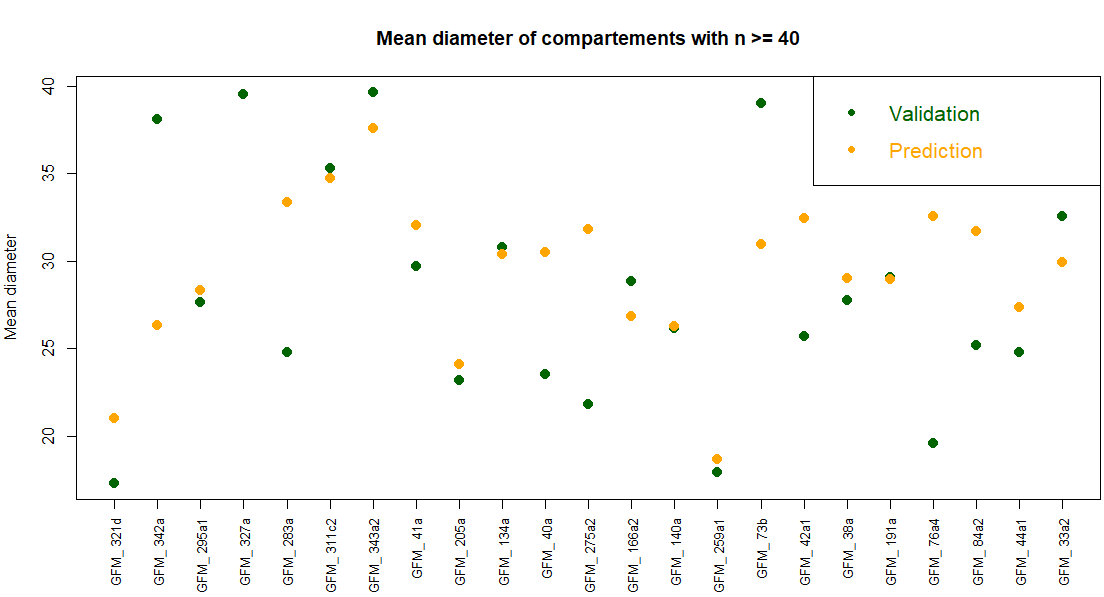
\includegraphics[scale = 0.4]{radius.png}
  \caption{Sampled mean diameter vs observed mean diameter for compartments with sufficient samples.}
  \label{fig:radius}
\end{figure}

\begin{table}[H]
\setlength\arrayrulewidth{1pt}
\centering
\begin{adjustbox}{max width=\textwidth}

\begin{tabular}{|c|c|c|}
\hline 
\rowcolor{Gray}
\textbf{Median} & \textbf{Mean} & \textbf{RSE} \\ 
\hline 
-2.8218 & -2.4574 & 5.487 \\ 
\hline 
\end{tabular} 

\end{adjustbox}

\caption{Summary Statistics of the observed diameter per compartment subtracted the mean sampled diameter}
\label{summary statistics}
\end{table}

The mean diameter is overestimated in the median and mean by 2.82cm and 2.46cm respectively. The residual standard error is 5.487cm.
\clearpage
\section{Discussion} 
% !TEX root = Master.tex

The objective of this study is to contribute to the development of LiDAR assisted forest inventories by developing
a statistical sound approach to derive unbiased diameter distribution models from LiDAR data for homogeneous
compartments of the forest. Prediction is successfully performed by a generalized linear
regression model using the gamma distribution with log as a link function. Clustering the compartments into three groups led to enough samples per cluster to
perform distribution engineering. Clustering is not meant to find groups upon a decision for more or less correction is made, but
to find an appropriate correction for similar compartments. Clustering further uncovered the issue of not detecting
equally height trees, which introduced additional bias in the tree diameter prediction. Bias correction is
achieved by fitting a gamma distribution on the diameter distribution of each cluster from the inventory dataset
and subsequently the predicted diameter distribution. A correction factor is calculated based on the ratio of the
shape and scale parameter of both fitted distributions for each cluster. High confidence is thus given to the
inventory dataset. Subsequently, the correction factor is applied for each section. \\

This approach could solve all present challenges, without relying on any heuristic methods apart from choosing
an appropriate amount of clusters and variables. Hence the objective of finding a statistical sound approach is achieved.\\

We could not find studies with similar approaches to the objective. 
The achieved residual standard error of the mean diameter of the corrected compartment distribution of 5.49cm (see Section \ref{Results}) is satisfying.
To compare and assess the modelling of the distribution, a inventory dataset of fully sampled compartments is necessary. 
The RSE could be further reduced by improving the tree species detection rate and likely crown area estimation. Comparing different amount of k cluster could be an interesting extension. 
The residual standard error of the regression model with 3.81cm is compared to another study. G. Liu, J. Wang, P. Dong, Y. Chen, Z. Liu (2018) [17] achieved a significantly better diameter residual standard error of 1.28 cm using solely LiDAR data. \textit{"Octree segmentation, connected component labelling and random Hough transform are comprehensively used to identify trunks and extract DBH of trees in sample plots."} \\

Nevertheless, this sophisticated approach can only be applied on plot level (small sampling location in a forest) and likely not scaled up on a whole forest. Ultimately, a residual standard error of below 5cm is satisfying. \\

The advantage of the presented approach is that an extension of the estimation of the unbiased tree diameter distribution based on just the LiDAR scanning system can be achieved, even though the majority of the area did not undergo any manual sampling activities.\\
Additionally, by making use of this bias correction attempt by fitting and adjusting parametric distributions instead of just relying on the predicted diameter distribution, outlier occurrences at the outer quantiles are no longer an issue (due to overestimated crown areas), meaning that overestimation of the tree diameter is also prevented. 




\clearpage



\addcontentsline{toc}{section}{Appendix}
\section*{Appendix} \label{Appendix}
% !TEX root = Master.tex

Include appendix here...

\clearpage

\addcontentsline{toc}{section}{References}
\section*{References}
%\subsection*{Literature}
% !TEX root = Master.tex

\noindent
[1] ForestEye Research GmbH und ARGUS Forstplanung, 2018: Handanweisung zur Betriebsinventur und
Forsteinrichtung in den Gräflich Bernstorff’schen Betrieben, Forstamt Gartow, Version 23.04.2018\\

\noindent
[2] Airborne laser scanning - an introduction and overview, 1999: Aloysius Wehr, Uwe Lohr, ISPRS Journal of
Photogrammetry and Remote Sensing. S. 68 - 82\\

\noindent
[3] Das Laserscanning. Eine neue Datenquelle zur Erfassung der Topographie, 2004: Karl Kraus, Paul
Dorninger, Wiener Schriften zur Geographie und Kartographie. S. 312 - 318.\\

\noindent
[4] On the distribution of a variate whose logarithm is normally distributed, 1941, Finney, D. J., Journal Royal Statiscal Society, v.7, p.155-161, 1941. Supplement.\\

\noindent
[5] Regression: Models, Methods and Applications. Berlin: Springer-Verlag. Ludwig Fahrmeir, Thomas Kneib, Stefan Lang, Brian Marx (2013) \\

\noindent
[6] Matching remotely sensed and field-measured tree size distributions. Jari Vauhkonen, Lauri Mehtätalob. Canadian Journal of Forest Research, 2015, 45(3): 353-363\\

\noindent
[7] Applied Multivariate Statistical Analysis (6th Edition), Richard A. Johnson, Dean W. Wichern. (02 April 2007)\\

\noindent
[8] factoextra: Extract and Visualize the Results of Multivariate Data Analyses, Alboukadel Kassambara and
Fabian Mundt, 2017, R package version 1.0.5 \\
https://CRAN.R-project.org/package=factoextra \\

\noindent
[9] jtools: Analysis and Presentation of Social Scientific Data, Jacob A. Long, 2018, R package version 1.1.1\\
https://cran.r-project.org/package=jtools \\

\noindent
[10] plotly: Create Interactive Web Graphics via plotly.js. R package version 4.7.1. Carson Sievert, Chris Parmer, Toby Hocking, Scott Chamberlain, Karthik Ram, Marianne Corvellec and
Pedro Despouy (2017). \\
https://CRAN.R-project.org/package=plotly \\

\noindent
[11] ggplot2: Elegant Graphics for Data Analysis. H. Wickham. Springer-Verlag New York, 2016 \\

\noindent
[12] Projektbericht: Orthobild-Mosaik und Airborne Laserscanning Forsteinrichtung Gartow, Marko Pilger, GEOCART, 06.11.2018, Version 1.0\\

\noindent
[13] Mathematical Methods of Statistics. Cramer, H. (1946) Princeton University Press, Princeton.\\

\noindent
[14]  Introduction to Mathematical Statistics, 4th edition. R. V. Hogg and A. T. Craig (1978) New York: Macmillan\\

\noindent
[15]  R.A. Fisher and the making of maximum likelihood 1912-1922. Aldrich, John. (1997). Stat Sci. 12. 10.1214/ss/1030037906. \\

\noindent
[16] fitdistrplus: An R Package for Fitting Distributions. Marie Laure Delignette-Muller, Christophe Dutang (2015).  Journal of Statistical Software, 64(4), 1-34.\\
 https://cran.r-project.org/web/packages/fitdistrplus/vignettes/paper2JSS.pdf\\

\noindent
[17] MDPI and ACS Style. Estimating Individual Tree Height and Diameter at Breast Height (DBH) from Terrestrial Laser Scanning (TLS) Data at Plot Level.
Liu, G.; Wang, J.; Dong, P.; Chen, Y.; Liu, Z. Forests 2018, 9, 398.\\





%\subsection*{R-Packages}
%% !TEX root = Master.tex

\noindent
[8] factoextra: Extract and Visualize the Results of Multivariate Data Analyses, Alboukadel Kassambara and
Fabian Mundt, 2017, R package version 1.0.5, \\https://CRAN.R-project.org/package=factoextra \\

\noindent
[9] jtools: Analysis and Presentation of Social Scientific Data, Jacob A. Long, 2018, R package version 1.1.1,
https://cran.r-project.org/package=jtools \\

\noindent
[10] Carson Sievert, Chris Parmer, Toby Hocking, Scott Chamberlain, Karthik Ram, Marianne Corvellec and
Pedro Despouy (2017). plotly: Create Interactive Web Graphics via plotly.js. R package version 4.7.1.
https://CRAN.R-project.org/package=plotly \\

\noindent
[11] H. Wickham. ggplot2: Elegant Graphics for Data Analysis. Springer-Verlag New York, 2016 \\

\noindent
[16] Marie Laure Delignette-Muller, Christophe Dutang (2015). fitdistrplus: An R Package for Fitting Distributions. Journal of Statistical Software, 64(4), 1-34.\\
 https://cran.r-project.org/web/packages/fitdistrplus/vignettes/paper2JSS.pdf\\





% MAKE THE REFERENCES PROPER; CITATIONS ETC....
	
\clearpage

\addcontentsline{toc}{section}{List of Figures}	
\listoffigures


\clearpage

\addcontentsline{toc}{section}{List of Tables}
\listoftables


\clearpage

\addcontentsline{toc}{section}{List of Abbreviations}
\section*{List of Abbreviations}
% !TEX root = Master.tex

\begin{acronym}

\acro{chm}[CHM]{Canopy Height Model}
\acro{dbh}[DBH]{Tree diameter (measured at 1.3m)}
\acro{gamlss}[GAMLSS]{Generalized Additive Model for Location Scale and Shape}
\acro{gis}[GIS]{Geographical Information System}
\acro{lm}[LM]{Linear Model}
\acro{glm}[GLM]{Generalized Linear Model}
\acro{lidar}[LiDAR]{Light Detection and Ranging}
\acro{ladar}[LADAR]{Laser Detection and Ranging}
\acro{gps}[GPS]{Global Positioning System}
\acro{rse}[RSE]{Residual Standard Error}
\acro{relse}[SE\%]{Relative Standard Error}
\acro{imu}[IMU]{Inertial Measurement Unit}
\acro{ci}[CI]{Confidence Interval}
\acro{rss}[RSS]{Sum of Squared Residuals} 
\acro{mle}[MLE]{Maximum Likelihood Estimation} 
\acro{aic}[AIC]{Akaike's Information Criterion} 
\acro{bic}[BIC]{Bayesian Information Criterion} 




\end{acronym}


\subsection*{Tree Species}
\begin{acronym}

\acro{bu}[Bu]{Beech} 
\acro{dgl}[Dgl]{Douglas fir}
\acro{ei}[Ei]{Oak}
\acro{fi}[Fi]{Spruce}
\acro{ki}[Ki]{Pine}
\acro{lae}[Lä]{Larch}
\acro{slh}[SLh]{Other Hardwood}
\acro{snh}[SNh]{Other Softwood}
\acro{ta}[Ta]{Fir}

\end{acronym}


\clearpage

	
\end{document}

